\documentclass[12pt, a4paper]{article} 
\documentclass[12pt, a4paper]{article} 
\usepackage{fontspec} % Font selection for XeLaTeX; see fontspec.pdf. 

\usepackage{xeCJK}	% 中文使用 XeCJK,利用 \setCJKmainfont 定義中文內文、粗體與斜體的字型
%\usepackage[BoldFont, SlantFont]{xeCJK}% 中文使用 XeCJK,並模擬粗體與斜體(\textbf{ } \textit{ })
\defaultfontfeatures{Mapping=tex-text} % to support TeX conventions like ``---''
\usepackage{xunicode} % Unicode support for LaTeX character names(accents, European chars, etc)
\usepackage{xltxtra} 						% Extra customizations for XeLaTeX
\usepackage{amsmath, amssymb}
\usepackage{enumerate}
\usepackage{graphicx, subfig, float, wrapfig} % support the \includegraphics command and options
\usepackage[outercaption]{sidecap} %[options]=[outercaption], [innercaption], [leftcaption], [rightcaption]
\usepackage{array, booktabs}
\usepackage{color, xcolor}
\usepackage{longtable}
\usepackage{colortbl}                          				
\usepackage{listings}						%直接將 latex 碼轉換成顯示文字
\usepackage[parfill]{parskip} 				% 新段落前加一空行,不使用縮排
%\usepackage{geometry} % See geometry.pdf to learn the layout options. There are lots.
\usepackage[left=1.5in,right=1in,top=1in,bottom=1in]{geometry} 

%-----------------------------------------------------------------
%  中英文內文字型設定
\setCJKmainfont							% 設定中文內文字型
	[
		BoldFont=Microsoft YaHei	% 定義粗體的字型(依使用的電腦安裝的字型而定)
	]
	{新細明體}							% 設定中文內文字型
\setmainfont{Times New Roman}				% 設定英文內文字型
\setsansfont{Arial}						% 無襯字字型 used with {\sffamily ...}
%\setsansfont[Scale=MatchLowercase,Mapping=tex-text]{Gill Sans}
\setmonofont{Courier New}				% 等寬字型 used with {\ttfamily ...}
%\setmonofont[Scale=MatchLowercase]{Andale Mono}
% 其他字型(隨使用的電腦安裝的字型不同,用註解的方式調整(打開或關閉))
% 英文字型
\newfontfamily{\E}{Calibri}				
\newfontfamily{\A}{Arial}
\newfontfamily{\C}[Scale=0.9]{Calibri}
\newfontfamily{\R}{Times New Roman}
\newfontfamily{\TT}[Scale=0.8]{Times New Roman}
% 中文字型
\newCJKfontfamily{\MB}{Microsoft YaHei}				% 適用在 Mac 與 Win
\newCJKfontfamily{\SM}[Scale=0.8]{新細明體}	% 縮小版新細明體
\newCJKfontfamily{\K}{標楷體}                	% Windows下的標楷體
% 以下為自行安裝的字型:CwTex 組合
%\newCJKfontfamily{\CF}{cwTeX Q Fangsong Medium}	% CwTex 仿宋體
%\newCJKfontfamily{\CB}{cwTeX Q Hei Bold}			% CwTex 粗黑體
%\newCJKfontfamily{\CK}{cwTeX Q Kai Medium}   		% CwTex 楷體
%\newCJKfontfamily{\CM}{cwTeX Q Ming Medium}		% CwTex 明體
%\newCJKfontfamily{\CR}{cwTeX Q Yuan Medium}		% CwTex 圓體
%-----------------------------------------------------------------------------------------------------------------------
\XeTeXlinebreaklocale "zh"             		%這兩行一定要加,中文才能自動換行
\XeTeXlinebreakskip = 0pt plus 1pt     		%這兩行一定要加,中文才能自動換行
%-----------------------------------------------------------------------------------------------------------------------
\newcommand{\cw}{\texttt{cw}\kern-.6pt\TeX}	% 這是 cwTex 的 logo 文字
\newcommand{\imgdir}{../images/}				% 設定圖檔的目錄位置
\renewcommand{\tablename}{表}					% 改變表格標號文字為中文的「表」(預設為 Table)
\renewcommand{\figurename}{圖}				% 改變圖片標號文字為中文的「圖」(預設為 Figure)

% 設定顏色 see color Table: http://latexcolor.com
\definecolor{slight}{gray}{0.9}				
\definecolor{airforceblue}{rgb}{0.36, 0.54, 0.66} 
\definecolor{arylideyellow}{rgb}{0.91, 0.84, 0.42}
\definecolor{babyblue}{rgb}{0.54, 0.81, 0.94}
\definecolor{cadmiumred}{rgb}{0.89, 0.0, 0.13}
\definecolor{coolblack}{rgb}{0.0, 0.18, 0.39}
\definecolor{beaublue}{rgb}{0.74, 0.83, 0.9}
\definecolor{beige}{rgb}{0.96, 0.96, 0.86}
\definecolor{bisque}{rgb}{1.0, 0.89, 0.77}
\definecolor{gray(x11gray)}{rgb}{0.75, 0.75, 0.75}
\definecolor{limegreen}{rgb}{0.2, 0.8, 0.2}
\definecolor{splashedwhite}{rgb}{1.0, 0.99, 1.0}

%---------------------------------------------------------------------
% 映出程式碼 \begin{lstlisting} 的內部設定
\lstset
{	language=[LaTeX]TeX,
    breaklines=true,
    %basicstyle=\tt\scriptsize,
    basicstyle=\tt\normalsize,
    keywordstyle=\color{blue},
    identifierstyle=\color{black},
    commentstyle=\color{limegreen}\itshape,
    stringstyle=\rmfamily,
    showstringspaces=false,
    %backgroundcolor=\color{splashedwhite},
    backgroundcolor=\color{slight},
    frame=single,							%default frame=none 
    rulecolor=\color{gray(x11gray)},
    framerule=0.4pt,							%expand outward 
    framesep=3pt,							%expand outward
    xleftmargin=3.4pt,						%to make the frame fits in the text area. 
    xrightmargin=3.4pt,						%to make the frame fits in the text area. 
    tabsize=2								%default :8 only influence the lstlisting and lstinline.
}
   % 使用自己維護的定義檔

% 文章開始
\title{ \XeLaTeX {\MB 外製圖形的引入}}
\author{{\SM 汪群超}}
\date{{\TT \today}} 	 
\begin{document}
\maketitle
\fontsize{12}{22pt}\selectfont
圖片在科技類文體扮演重要的角色,而這些圖形須經由其他軟體產生,然後被安置在文件的適當位置。如同表格的製作,有些套件被設計來置入圖形,本文介紹其中較常用的 graphicx 套件。而圖形檔的型態最常見的有 EPS/JPG/PNG/PDF 等格式。傳統的 \LaTeX 文件慣用 EPS 圖檔,這種所謂的「描邊圖檔」非常適合數學或統計圖,可以為圖形加上文字或其他線條,檔案小而且清晰。近二十年,因為網路興起及多媒體的表現日漸重要,才有壓縮圖檔的出現,其中以 JPG 圖檔最為流行,適合各種靜態圖形與相片。\XeLaTeX 改善了原先 \LaTeX 對圖格式的不夠友善,讓不同格式的圖檔可以相容並存,無疑是使用 \LaTeX 者的福音。本章介紹圖形的安插方式。

圖 \ref{fig:scale} 將一個名為  \textit{distribution\_1.jpg} 的圖檔放在頁面的中央。與表格類似,圖形環境指令 $\backslash begin\{figure\}$ 可以用來控制圖形所在的位置。請注意預設的圖形檔路徑與文章相同,圖形若不是放置於此,必須指定完整的路徑。譬如\footnote{請利用  TexMaker 編譯本文,並同時下載本文所使用的所有圖檔。下載並解壓縮後,請將檔案  distribution\_1.jpg 拷貝到與本文相同目錄。其餘圖檔留在子目錄  images 裡。}

%\begin{center}\colorbox{slight}{\begin{tabular}{p{0.9\textwidth}}
%	{\A $\backslash$includegraphics\{d:/MyTex/images/distribution\_1.jpg\}}
%\end{tabular}}\end{center}
\bigskip
	\begin{lstlisting}
		\includegraphics{d:/MyTex/images/distribution_1.jpg}
	\end{lstlisting}
\bigskip

\begin{figure}[h]
    \centering
        \includegraphics[scale=0.5]{distribution_1.jpg}
    \caption{利用 scale 選項將原圖縮小 0.5 倍( JPG 圖)}
    \label{fig:scale}
\end{figure}


當然如果一份文件中引入許多分散在不同目錄的圖檔,勢必相當麻煩,因此將所有檔案都集中到預設的目錄,也不失是個好方法。另一個麻煩是,當這份文件可能會在不同的電腦編譯時,如果兩部電腦的目錄不一致,那還是行不通的,終究得改來改去,不如統一放在某個固定目錄裡,譬如與文章同層的子目錄。為避免在指令中放在冗長得完整路徑,一般會在定義區設定一個路徑命令,用來縮短指令所需的長度,另提供彈性更動目錄的方便。譬如,本文在定義區設定以下的新命令:

%\begin{center}\colorbox{slight}{\begin{tabular}{p{0.9\textwidth}}
%	{\A $\backslash$newcommand\{$\backslash$imgdir\}\{images/\}}
%\end{tabular}}\end{center}
\bigskip
	\begin{lstlisting}
		\newcommand{\imgdir}{images/}	
	\end{lstlisting}

這個新命令自訂為  $\backslash$imgdir ,定義了一個與編譯文章路徑相同的子目錄:images,也就是所有圖形檔案放置的目錄。使用的方式為 \footnote{本文字第二張圖片開始,採用這個方式,請對照 TEX 檔}

%\begin{center}\colorbox{slight}{\begin{tabular}{p{0.9\textwidth}}
%	{\A $\backslash$includegraphics\{$\backslash$imgdir\{distribution\_1.eps\}\}}
%\end{tabular}}\end{center}
\bigskip
	\begin{lstlisting}
		\includegraphics{\imgdir distribution_1.jpg}	
	\end{lstlisting}
	
另外,圖形的大小不見得適合放在想放置的位置,有必要作縮小或甚至放大。圖 \ref{fig:scale}  利用  scale 選項原圖縮小 0.5 倍,而圖 \ref{fig:width} 利用 width 選項原圖縮小為內文行寬的 0.8 倍。調整時長寬依等比例縮放。\\

\begin{figure}[H]
    \centering
    \includegraphics[width=0.8\textwidth]{\imgdir distribution_1.eps}
    \caption{利用 width 選項將原圖調整為內文行寬的 0.8 倍(EPS 圖)}
    \label{fig:width}
\end{figure}

\begin{wrapfigure}{R}{0.4\textwidth}
\centering
\includegraphics[width=0.4\textwidth]{\imgdir XeTex.PNG}
\caption{文繞圖示範}\label{fig:PNG}
\end{wrapfigure}

圖 \ref{fig:scale} 與圖  \ref{fig:width} 是從 MATLAB 軟體產生的同一張圖,只是儲存時選擇的檔案型態不一樣。圖 \ref{fig:scale} 是 JPG 檔,圖  \ref{fig:width} 則是 EPS 檔。從圖的外觀很容易判斷 EPS 圖檔非常清晰,適合數學圖形的表現。而 {\C JPG} 圖檔因為壓縮的關係,造成失真,適合用在螢幕截圖或是一般照片的呈現。圖 \ref{fig:PNG} 是一張電腦螢幕截圖,儲存成 PNG 檔,也順便展示了文繞圖的技巧。這當然需要動用到特別的套件:wrapfig。

圖形為配合文字與版面的配置,有時候可以將編號與說明文字拉到左側或右側,如圖 \ref{fig:side} 所示。這個功能使用了套件 sidecap。
\begin{SCfigure}[0.9][h]  % 數字 0.9 代表圖形開始的位置
\caption{標號與說明文字在側邊的示範}
\includegraphics[width=0.4\textwidth]{\imgdir XeTex.PNG}
\label{fig:side}
\end{SCfigure}



%\begin{figure}[H]
%    \centering
%        \includegraphics{\imgdir{XeTex.PNG}}
%    \caption{螢幕截圖存成{\C PNG} 圖檔}
%    \label{fig:PNG}
%\end{figure}
圖 \ref{fig:JPG} 是另一張螢幕截圖,但存成 JPG 圖。圖 \ref{fig:angle} 進一步利用 angle 選項將原圖逆時鐘方向旋轉 30 度,同時將圖形的長寬做不等比例的設定。圖 \ref{fig:parallel} 則是將兩圖並列,使用了 subfig 的套件,圖形會自動編上 (a) 與 (b) 的標示,個別圖形還可以做文字說明,當然也可以省略。

\begin{figure}[h]
    \centering
        \includegraphics[scale=0.3]{\imgdir TexMaker.jpg}
    \caption{螢幕截圖存成 JPG 圖檔}
    \label{fig:JPG}
\end{figure}

 

\begin{figure}[H]
    \centering
        \includegraphics[angle=30,width=15cm, height=10cm]{\imgdir mv_min_7.eps}
    \caption{利用angle選項將原圖逆時鐘方向旋轉 30 度,同時將圖形的長寬做不等比例的設定。}
    \label{fig:angle}
\end{figure}

\begin{figure}[H]
    \centering
        \subfloat[$\beta$ 分配族群]{
        \includegraphics[scale=0.35]{\imgdir dist_5.eps}}
        \subfloat[不同自由度的 T 分配與標準常態]{
        \includegraphics[scale=0.35]{\imgdir dist_28.eps}}
    \caption{圖形並排的作法}
    \label{fig:parallel}
\end{figure}

在編輯含圖檔的文件中,常發生圖形在編輯後的位置與原先設定不同。原因通常是該頁剩餘空間不足以擺放圖形,此時 \LaTeX 會自動調整圖形的位置。大部分時候這樣的調整是可以接受的,但有時候會引發一連串圖形的位置與本文越離越遠,這當然是不恰當的。在圖形的設定中允許使用者指定位置,譬如指令

%\begin{center}\colorbox{slight}{\begin{tabular}{p{0.9\textwidth}}
%	{\C $\backslash$begin\{figure\}[h]}
%\end{tabular}}\end{center}
\bigskip
	\begin{lstlisting}
		\begin{figure}[h]
	\end{lstlisting}
\bigskip
後面方框中的 h 指的是 here,其他選擇如  [t] 指 top。這樣的選項只有建議權,常常被系統忽略,導致圖形的位置與自己的理想有差距。為避免這個情況的發生,希望取得多一點主導權,可以使用套件 float,並在設定圖形時使用  [H],也是 here 的意思,但採用大寫的  H 代表真正的主導權。不過雖然搶回主導權,將圖片放在自己囑意的位置,但要謹慎使用,切勿濫用,因為自己的排版功力不足時,往往會適得其反。

\begin{minipage}{.4\linewidth}
{\A minipage} 是另一種控制圖形位置的方式,適合必須與文字密切貼近的圖形。讓文字描述圖形時,可以用左圖或右圖,而不是依賴圖形編號。譬如,右圖示範的圖檔格為 PDF。此時,因為不能用 \verb|\begin{figure}|,沒有{\A label} 與  {\A caption}。

\end{minipage}
\begin{minipage}{.6\linewidth}
        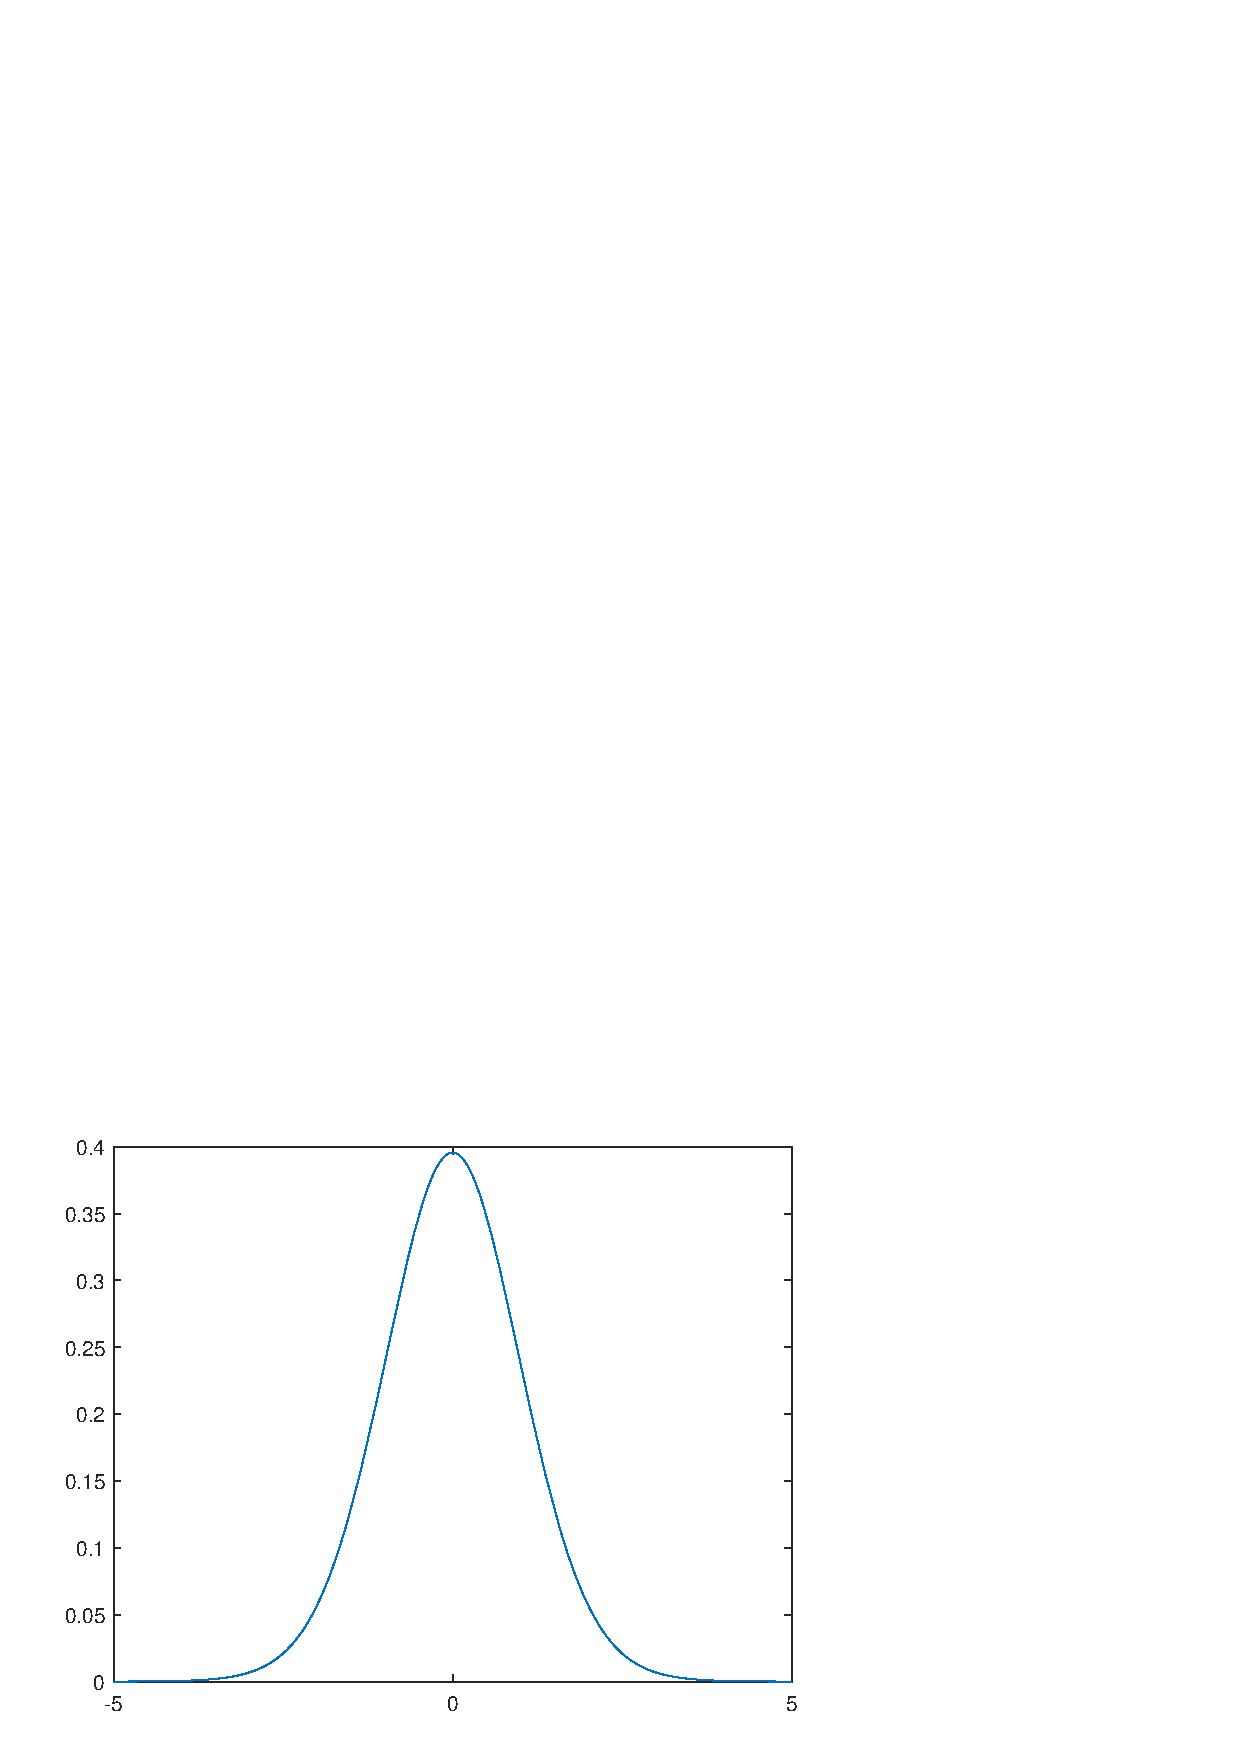
\includegraphics[scale=0.3]{test.pdf}
\end{minipage}
\end{document}
